\documentclass{amsart}
\usepackage{master}
\begin{document}
\title{Geometry and algebra of pseudo-holomorphic curves}
\author{Lectures by Professor John Pardon\\
Notes by Jackson Van Dyke}
\thanks{All errors introduced are my own.}
\date{June 20-22, 2018}
\maketitle

Pseudo-holomorphic curves were 
introduced by Gromov in 1985, and have become perhaps the central
tool in symplectic topology/geometry.

\section{Introduction to symplectic geometry}

\begin{defn}
A symplectic form on a manifold $M^{2n}$
is a closed $2$-form $\om$ which, when viewed as a pairing
$\om:TM\tp TM\fromto \RR$, is non-degenerate
(i.e. the induced map 
$TM\fromto \rdual{TM}$ is an isomorphism.)
and skew-symmetric.
\end{defn}

\begin{exm}
$\RR^{2n}$ with standard basis
$\left\{ x_1 , \cdots , x_n , y_1 , \cdots , y_n \right\}$
is a symplectic manifold with the symplectic form
\begin{equation}
\om_\std \ceqq \sum_{i = 1}^n 
\d{s_i} \ext \d{y_i}
\end{equation}
\end{exm}

\begin{thm}[Darboux]
For any symplectic manifold $M$ and point $p\in M$, 
there exists a function $f:U\fromto M$, (diffeomorphic onto its image),
where $U\subeq \RR^{2n}$ is open, $p\in f\left( u \right)$, and
$f^*\left( \om_M \right)  = \om_\std$.
\end{thm}

Define the symplectomorphisms 
$\Diff_0\left( M , \om \right)$ 
to consist of the diffeomorphisms
preserving the symplectic form.
Of course this is contained inside $\Diff_0\left( M  , \om^n \right)$, 
which are volume preserving.
Explicitly, the symplectomorphisms consist of the identity component of
\begin{equation}
\left\{ f:M\fromto M \st f^* \om = \om \right\}_0
\subeq 
\left\{ f:M\fromto M \st f^*\left( \om^n \right)= \om^n \right\}
\end{equation}

\begin{thm}[Gromov]
With respect to the $C^0$-topology, 
the inclusion of symplectomorphisms inside the volume preserving
diffeomorphisms is either closed or dense.
\end{thm}

If we have that this inclusion is closed, is somehow considered to be
the rigidity regime, and similarly, this inclusion being dense is somehow
considered to be the flexibility regime.

A \emph{symplectic embedding}
$f: \left( U , \om_n \right) \fromto \left( V, \om_V \right)$ is a map
(diffeomorphism onto its image) such that $f^* \om_V= \om_U$.
We introduce the following notation:
\begin{align}
\Ball^{2n}\left( r \right) & <
\left\{ \left( x_1 , \cdots , x_n , y_1 , \cdots , y_n \right) \in \RR^{2n}\st
\sum x_i^2 + y_i^2\leq r^2\right\}\\
\Ball^2\left( R \right) \times \RR^{2n-2} & <
\left\{ \left( x_1 , \cdots , x_n , y_1 , \cdots, y_n \right) \st
x_1^2 + y_1^2 \leq R^2\right\}
\end{align}

\begin{thm}
If there exists a symplectic embedding:
\begin{equation}
\Ball^{2n}\left( r \right) \inj \Ball^2\left( R \right) \times \RR^{2n-2}
\end{equation}
as in \cref{fig:non_squeeze}, then $r\leq R$.
\label{thm:non_squeeze}
\end{thm}

\begin{figure}
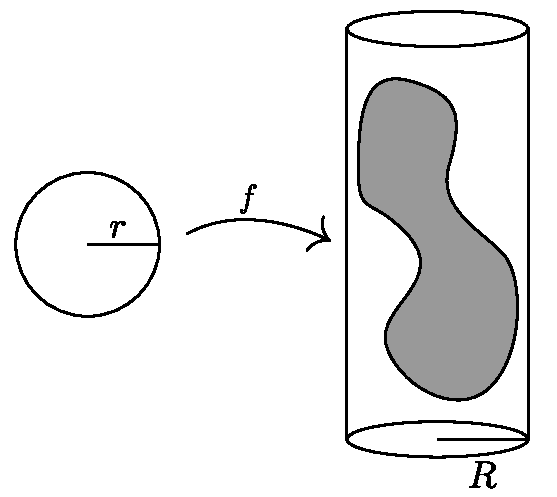
\includegraphics[width=0.4\textwidth]{non_squeeze.pdf}
\caption{If we have a symplectic embedding of a sphere inside 
a cylinder, then the radius of the cylinder must be larger than the radius of the 
sphere by \cref{fig:non_squeeze}.}
\label{fig:non_squeeze}
\end{figure}

Eliashberg, Conley-Zehnder, and Gromov all independently showed this.
Gromov's proof is the one that uses holomorphic curves, so we will focus more on this.

\subsection{Pseudo-holomorphic curves}

To prove \cref{thm:non_squeeze} we introduce the following notions:

\begin{defn}
An almost complex structure (acs) on $M^{2n}$ is an endomorphism 
$J:TM\fromto TM$ such that $J^2 = -\id$.
\end{defn}

Equivalently this is putting the structure of a $\CC$ vector space 
on $TM$, and then $J$ is just multiplication by $i$.

\begin{wrn}
Such an $\left( M , J \right)$ is \emph{NOT} in general locally
isomorphic to $\CC^n$.
\end{wrn}

An acs $J$ is said to be tamed by $\om$ iff
$\om\left( v , J v \right) > 0$, for all
$v\in TM \minus\left\{ 0 \right\}$.
$J$ is said to be compatible with $\om$ iff
$\left( v , w \right)\mapsto \om\left( v , Jw \right)$ is a Riemannian metric, 
that is, it is symmetric and positive definite.

\begin{lem}
Compatible implies tame.
\end{lem}

Often times compatibility is more convenient, so people just work with this 
assumption instead.

\begin{lem}
On a symplectic vector space $\left( V , \om \right)$, 
the spaces of compatible (resp. tame) $J$
are contractible.
\end{lem}

A pseudo-holomorphic curve is a holomorphic map 
\begin{equation}
u:\left( C , j \right) \fromto \left( M , J \right)
\end{equation}
where $\left( C ,j \right)$ is a Riemann surface and $du:TC\fromto u^*TM$
is $\CC$-linear.

\begin{proof}[Proof of \cref{thm:non_squeeze}]
WLOG, $\im\left( f \right)$ is contained in a compact subset of
$\Ball^2\left( R \right) \times \RR^{2n-2}$. 
To see this, just restrict $f$ to $\Ball^{2n}\left( r - \e \right)$, where
$r - \e \leq R$ for all $\e > 0$, then $r \leq R$.
Since $\im\left( f \right)$ is compact, it gives an embedding
\begin{equation}
f:\Ball^{2n}\left( r \right) \inj \Ball^2\left( R \right) \times
\left( \RR^{2n-2} / N \ZZ^{2n-2} \right)
\end{equation}
for large $N < \infty$.
We now write $\RR^{2n - 2} / N\ZZ^{2n - 2} = T^{2n-2}$, and further embed:
\begin{equation}
\Ball^2\left( R \right) \times
\left( \RR^{2n-2} / N \ZZ^{2n-2} \right)
\inj S^2 \times T^{2n-2}
\end{equation}
where $S^2$ is the sphere of the same area as $\Ball^2\left( R \right)$.
All together, we have a symplectic embedding:
\begin{equation}
f: \Ball^{2n}\left( r \right)\inj \left(S^2 \times T^{2n-2},
\om_{S^2} + \om_{T^{2n-2}}\right)
\end{equation}
and want to show $r \leq R$.

Now equip $S^2 \times T^{2n-2}$ with a product acs
$J = J_{S^2} \dsum J_{T^{2n-2}}$, so it is biholomorphic to
$\CP^2 \times \left( \CC^{n-1} / \ZZ^{2n-2} \right)$ as a complex manifold.
Now consider the space
\begin{equation}
\cM_{0,1}\left( S^2 \times T^{2n-2} , J \right)
\ceqq
\left\{ u: \CP^1 \fromto S^2 \times T^{2n-2} \st
\d{u} \text{ is } \CC \text{ linear }\right\} / \sim
\end{equation}
where we have defined the relation:
\begin{equation}
u\sim u\comp \phi \st \phi 
\iff \CP^1 \fromto \CP^1, \phi\left( 0 \right) = 0
\end{equation}
So we are effectively quotienting out by the
$\PGL_2 \CC$ action on such maps, as long as they fix a point.

So if we have a map
\begin{equation}
u:\CP^1 \fromto \CP\times\left( \CC^{n-1} / \ZZ^{2n-2} \right)
\end{equation}
this splits as:
\begin{align}
u_1:\CP^1 \fromto \CP^1
&&
u_2:\CP^1 \fromto \CC^{n-1} / \ZZ^{2n-2}
\end{align}
We always get a lift as follows:
\begin{equation}
\begin{tikzcd}
\CP^1 \arrow{r}\arrow[dashed]{dr}{\text{lift}}&
\CC^{n-1} / \ZZ^{2n-2}\\
& \CC^{n-1}\arrow{u}
\end{tikzcd}
\end{equation}
since $\pi_1\left( \CP^1 \right) = 0$.
Therefore by Liouville's theorem, $u_2$ is constant.

We have a foliation by holomorphic $\CP^1$ as in \cref{fig:foliation}.
\begin{figure}
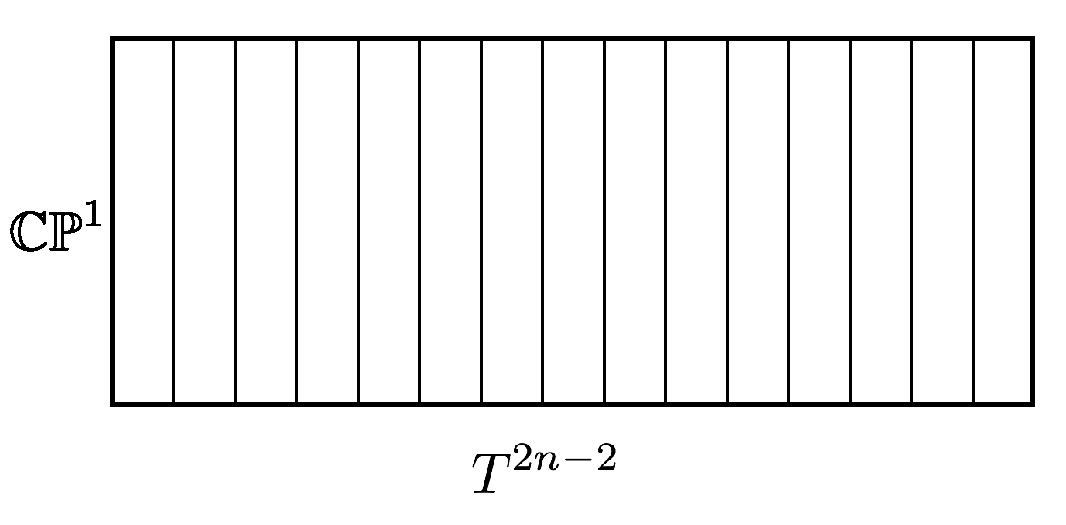
\includegraphics[width=0.5\textwidth]{foliation.pdf}
\caption{Foliation by holomorphic $\CP^1$.}
\label{fig:foliation}
\end{figure}

Now we have that
\begin{equation}
\cM_{0,1}^d\left( S^2 \times T^{2n-2} \right) \subeq
\cM_{0,1}\left( S^2 \times T^{2n-2} \right)
\end{equation}
is the set of curves $u$ with
$u_*\left[ \CP^1 \right] = d\left[ S^2 \right] \times \pt$.
In particular, we focus on $\cM_{0,1}^1\left( S^2 \times T^{2n-2} \right)$, 
which is just the total space
$S^2 \times T^{2n-2}$.
Moreover, this map is simply the evaluation map sending a curve
with a marked point to the image of the marked point.

In \cref{fig:fibers}, we can see the 
holomorphic curves with respect to
\begin{equation}
J_0 = J_{\CP^1} \dsum J_{\CC^{n-1} / \ZZ^{2n-2}}
\end{equation}
along with the holomorphic curves with respect to
$J_1$, which is some compatible acs on
$S^2 \times T^{2n-2}$ which agrees with $f_* J_\std$ over $\im \left( f \right)$.

\begin{figure}
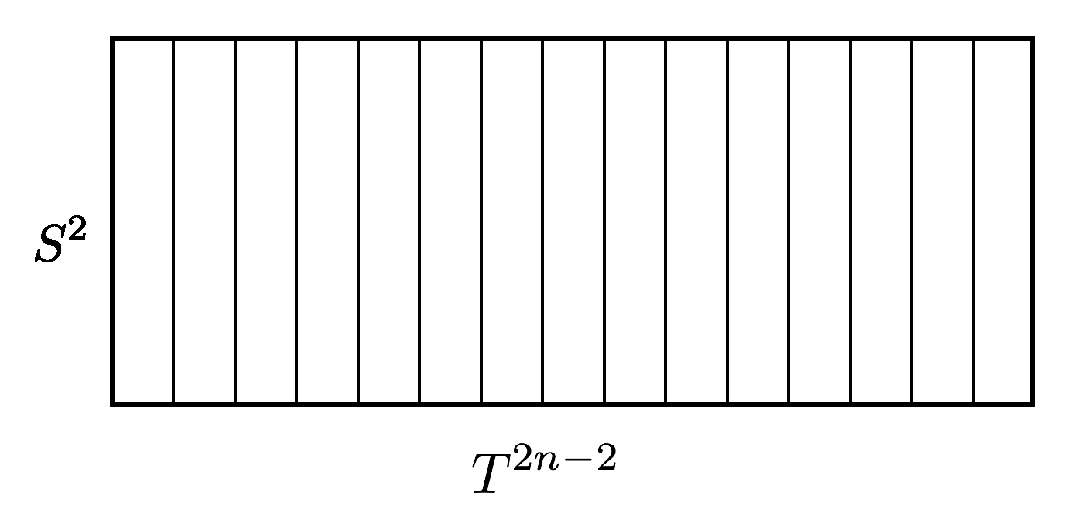
\includegraphics[width=0.5\textwidth]{fibers1.pdf}
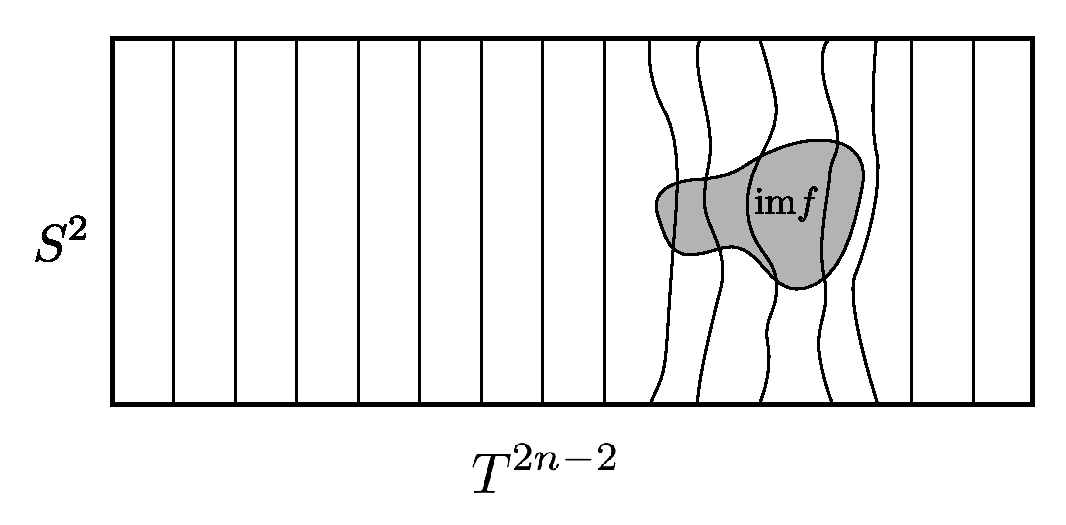
\includegraphics[width=0.5\textwidth]{fibers2.pdf}
\caption{Holomorphic curves with respect to $J_0$ and $J_1$.}
\label{fig:fibers}
\end{figure}

It is a classical result that the space of $\om$-compatible almost-complex
structures is nonempty and contractible.
Therefore we can choose a path of complex structures
$\left\{ J_t \right\}_{t\in \left[ 0,1 \right]}$ between $J_0$ and $J_1$.
Now the collection of $t\in \left[ 0,1 \right]$, such that $1$-pointed
genus $0$, curve in $S^2 \times T^{2n-2}$ with respect to $J_t$
in class $\left[ S^2 \right] \times \pt$ projects as
\begin{equation}
\begin{tikzcd}
\cM_{0,1}^1\left( S^2\times T^2, \left\{ J_t \right\}\right)
\arrow{d}{\pi}\\
\left[ 0,1 \right]
\end{tikzcd}
\end{equation}

Now we know $\pi^{-1}\left( 0 \right) = S^2 \times T^{2n-2}$, but we don't
know much more besides this. 
To continue, we need to appeal to some big non-trivial results about moduli spaces
of holomorphic curves:
\begin{enumerate}
\item Gromov compactness: $\pi$ is proper (i.e. $\pi^{-1}$ of compact is compact)
\item For generic choice of $J_1$ and $\left\{ J_t \right\}_t$, the total space
$\cM_{0,1}^1\left( S^2 \times T^{2n-2} , \left\{ J_t \right\} \right)$
is a manifold with boundary $\pi^{-1}\left( - \right) \un \pi^{-1}\left( 1 \right)$.
Schematically, we have something like in \cref{fig:cobordism}.
\begin{figure}
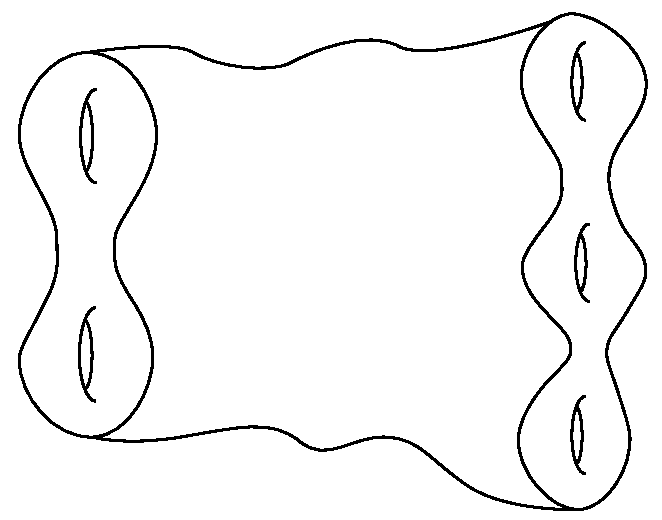
\includegraphics[width=0.3\textwidth]{cobordism.pdf}
\caption{Schematic of the space which is projected onto the interval $\left[ 0,1 \right]$.}
\label{fig:cobordism}
\end{figure}
To show this, we need transversality and non-linear Fredholm theory.
\end{enumerate}
Now consider the evaluation map
\begin{equation}
\ev: \cM_{0,1}^1\left( S^2 \times T^{2n-2} , \left\{ J_t \right\} \right) \fromto
S^2 \times T^{2n-2}
\end{equation}
We know $\ev_*\left[ \pi^{-1}\left( 0 \right) \right] = \left[ S^2 \times T^{2n-2} \right]$, 
but we have this cobordism, so actually
$\ev_*\left[ \pi^{-1}\left( 1 \right) \right] = \ev_*\left[ \pi^{-1}\left( 0 \right) \right]$.
In particular, this implies that
\begin{equation}
\ev: \cM_{0,1}^1\left( S^2 \times T^{2n-2} , J_1 \right) \fromto
D^2 \times T^{2n-2}
\end{equation}
is surjective.

Consider a holomorphic curve 
$u: \CP^1  \fromto S^2 \times T^{2n-2}$
which passes through $f\left( 0 \right)$
where $f$ is our embedding.
We have therefore actually produced a curve 
$v:\Sigma \fromto \Ball^{2n}\left( r \right)$ passing through the origin, where 
$\Sigma$ is as in the following diagram:
\begin{equation}
\begin{tikzcd}
\Sigma \ceqq u^{-1}\left( f\left( \Ball^{2n}\left( r \right) \right) \right)\arrow[hook]{r}
\arrow{d}{v}&
\CP^1\arrow{d}{u}\\
\Ball^{2n}\left( r \right)\arrow[hook]{r}{f}&
S^2 \times T^{2n-2}
\end{tikzcd}
\end{equation}
where $v$ is proper, since it is the pullback of the proper map $u$.
The picture here is as in \cref{fig:curve_v}.
\begin{figure}
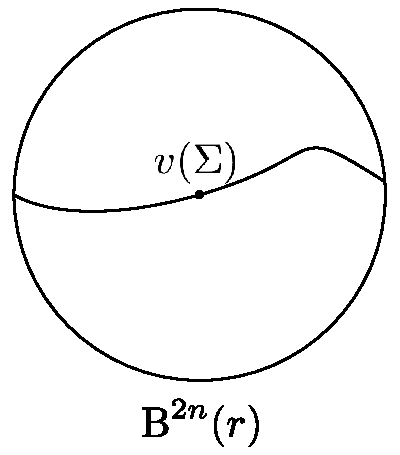
\includegraphics[width=0.3\textwidth]{curve_v.pdf}
\caption{The curve $v\left( \Sigma \right)$ on $\Ball^{2n}\left( r \right)$.}
\label{fig:curve_v}
\end{figure}
Now we have the following inequalities:
\begin{align}
\Area\left( v\left( \Sigma \right) \right)
&= \int_\Sigma v^* \om \\
&\leq \int_{\CP^1} u^* \om \\
&= \lr{u_*\left[ \CP^1 \right] , \left[ \om \right]} \\
&= \Area\left( S^2 \right) 
= \Area\left( \Ball^2\left( R \right) \right) = \pi R^2
\end{align}
Now the last ingredient is the following:
\begin{prop}[Monotonocity]
If $v: \Sigma \fromto \Ball^{2n}\left( r \right)\subeq \CC^n$ is a proper, non-constant,
holomorphic (with respect to $J_\std$) map covering the origin, then
\begin{equation}
\int_\Sigma v^* \om \geq \pi r^2
\end{equation}
\label{prop:monotonicity}
\end{prop}
\begin{proof}[Sketch proof 1 of \cref{prop:monotonicity}]
Observe a holomorphic curve in $\CC^n$ is a minimal surface, (actually this is true only under
the assumption that this is a minimal embedding rather than holomorphic.)
\end{proof}
\begin{proof}[Proof 2 of \cref{prop:monotonicity}]
We have our standard form:
\begin{equation}
\om_\std \ceqq
\sum_i \d{x_i} \ext \d{y_i} = \d{\lam_\std}
\end{equation}
which has a standard primitive:
\begin{equation}
\lam_\std = \sum_i
\frac{1}{2} \left( x_i \d{y_i} - y_i \d{x_i}  \right)
\end{equation}
now define
\begin{equation}
F\left( t \right) \ceqq 
\frac{1}{t^2} 
\int_{V^{-1}\left( \Ball^{2n}\left( t \right) \right)}
v^* \om = \frac{1}{t^2}\left[ \Area\left( v\left( \Sigma \right)\cap 
\Ball^{2n}\left( t \right)\right) \right]
\end{equation}
Now it is enough to just prove $F$ is increasing, since
\begin{equation}
\lim_{t\fromto 0^+} F\left( t \right) = 
\pi \left( \text{ order of vanishing of } v \text{ at } 0 \right)
\end{equation}
To see this we can calculate:
\begin{equation}
F\left( t \right) = \frac{1}{t^2} \int v^*\left( d\lam \right) = 
\frac{1}{t^2} \int_{v^{-1}\left( \p \Ball^{2n}\left( t \right) \right)}
v^* \lam_\std
\end{equation}
where we have used Stokes theorem.
Now we use coordinates
\begin{equation}
\begin{cd}
\RR_s\times S_m^{2n-1}\arrow{r}&
\RR^{2n}\minus 0 \\
\left( s,m \right)\arrow[mapsto]{r}&
e^{s/2} m
\end{cd}
\end{equation}
In these coordinates, $\lam_\std = e^s \al_\std$ where
\begin{equation}
\al_\std \ceqq \restr{\lam_\std}{\text{unit } S^{2n-1}}
\end{equation}
Then we can pick up this calculation from above:
\begin{equation}
F\left( t \right) = \frac{1}{t^2}
\int v^*\left( t^2 \al_\std \right) = 
\int_{V^{-1}\left( \p \Ball^{2n}\left( t \right) \right)}
v^*\left( \al_\std\right)
\end{equation}
Now we can use Stokes theorem again to get:
\begin{equation}
F\left( t_1 \right) - F\left( t_2 \right) = 
\int_{v^{-1}\left( \Ball^{2n}\left( t_1 \right)\minus
\Ball^{2n}\left( t_2 \right)\right)}
v^*\left( d \al_\std \right)
\end{equation}
Finally we can calculate that $d\al_\std$ is $\geq 0$ on complex lines, so the RHS
is nonnegative since $v$ is holomorphic.
\end{proof}
The result clearly follows from \cref{prop:monotonicity}.
\end{proof}

\section{Non-linear Fredholm theory for moduli of pseudo-holomorphic curves}

Let $\left( X , J \right)$ be an almost complex manifold, and let
$\left( C , j \right)$ be a closed Riemann surface.
E.g. $\CP^1$ or $T^2$. 
More generally, we will allow for $C$ to have nodes (locally $\left\{ xy = 0 \right\}$) but
to keep the discussion simple, we won't talk much about this.
Then we have the associated moduli space:
\begin{equation}
\cM\left( C , X \right) \ceqq
\left\{ u:C\fromto C \st \d{u} \CC\text{-linear}, u \in \cC^\infty \right\}
\end{equation}
We can always write:
\begin{equation}
\d{u} = \frac{1}{2}\left( \d{u} + J \comp \d{u} \comp j \right)+
\frac{1}{2}\left( \d{u} - J \comp \d{u} \comp j \right)
= \ubr{\left( \d{u} \right)^{0,1}}{\CC\text{-antilinear}} + 
\ubr{\left( \d{u} \right)^{1,0}}{\CC\text{-linear}}
\end{equation}
Our equation $\left( \d{u} \right)^{0,1} = 0$ is elliptic.
Elliptic regularity just means $u\in C^2$ implies $u\in C^\infty$. 

Now consider the $k,p$ maps:
\begin{equation}
W^{k,p} = \left\{ 
f \text{ distribution on } \RR^n \st
\forall \abs{\al} \leq k, 
D^\al f \in L^p \right\}
\end{equation}
We can think of this as the completion of $C^\infty_c\left( \RR^n \right)$
with respect to 
\begin{equation}
\norm{f}_{k,p}\ceqq \sum_{\abs{\al} \leq k} \norm{D^\al f}_p
\end{equation}
How do we generalize this to $W^{k,p}\left( C ,X \right)$?
We can think of this two ways:
\begin{enumerate}
\item Well we can embed $X\subeq \RR^N$, and then
\begin{equation}
W^{k,p}\left( C , X \right)\subeq 
W^{k,p}\left( C , \RR^N \right)
\end{equation}
is the set of maps $f$ which almost everywhere land in $C$.

\item (This second definition only makes sense when $W^{k,p}\subeq C^0$.)
We can view $W^{k,p}\left( C , X \right) \subeq C^0\left( C , X \right)$ as the 
set of functions $f:C\fromto X$ which are locally of class $W^{k,p}$
with respect to the smooth atlases on $C$ and $X$.
\begin{equation}
\begin{tikzcd}
&C\arrow{r}{f}&X&\\
\RR^2\arrow[hook]{r}&
U\arrow{u}{\phi}\arrow{r}{\psi^{-1}f \phi}&
V\arrow{u}{\psi}&
\RR^{2n}\arrow[hook]{l}
\end{tikzcd}
\end{equation}
Then $\psi^{-1} f \phi \in W^{k,p}$.
\end{enumerate}

We now assume $W^{k,p}\left( C , X \right)$ is a smooth Banach manifold.
The charts are, for $u\in C^\infty\left( C , X \right)$, 
\begin{equation}
\begin{tikzcd}
W^{k,p}\left( C , u^* TX \right)
\arrow{r}&
W^{k,p}\left( C , X \right) \\
\xi\arrow[mapsto]{r}& \exp_u \xi
\end{tikzcd}
\end{equation}
Note that
$W^{k,p}\left( C , u^* TX \right)$ is
well defined since the pullback $u^*$ is a smooth bundle.
This is really true for any map
$\exp:TX\fromto X$ whose derivative at the zero section is $\id$. 
If we wanted to check if the transition maps between two of these are smooth, we would
just write down the following:
\begin{equation}
\begin{cd}
W^{k,p}\left( C , u^* TX \right)\arrow{r}&
W^{k,p}\left( C , X \right)&
W^{k,p}\left( C , v^* TX \right)\arrow{l}
\arrow[bend right=12pt,"\exp_v^{-1} \comp \exp_u: u^* TX\fromto v^* TX"']{ll}
\\
\xi\arrow[mapsto]{r}&
\exp_u \xi&\\
& \exp_v \eta& \eta \arrow[mapsto]{l}
\end{cd}
\end{equation}

Similarly, there is a bundle 
$\cE \fromto W^{k,p}\left( C , X \right)$ where
\begin{equation}
\cE = \bun_{u\in W^{k,p}\left( C , X \right)}
W^{k-1,p}\left( C,
\barr{\Hom}_\CC\left( TC , u^* TX \right)
\right)
\end{equation}
Note that 
$\barr{\Hom}_\CC\left( TC , u^* TX \right)$ denotes the
$\CC$ anti-linear maps $TC\fromto u^* TX$.
The sections of $\cE\fromto W^{k,p}\left( C , X \right)$ 
map $u\mapsto \left( \d{u} \right)^{0,1} = \barr{\p}\left( u \right)$.
The section measures how much these maps fail to be holomorphic.
The picture to have in mind is as in \cref{fig:sections_of_W}.
\begin{figure}
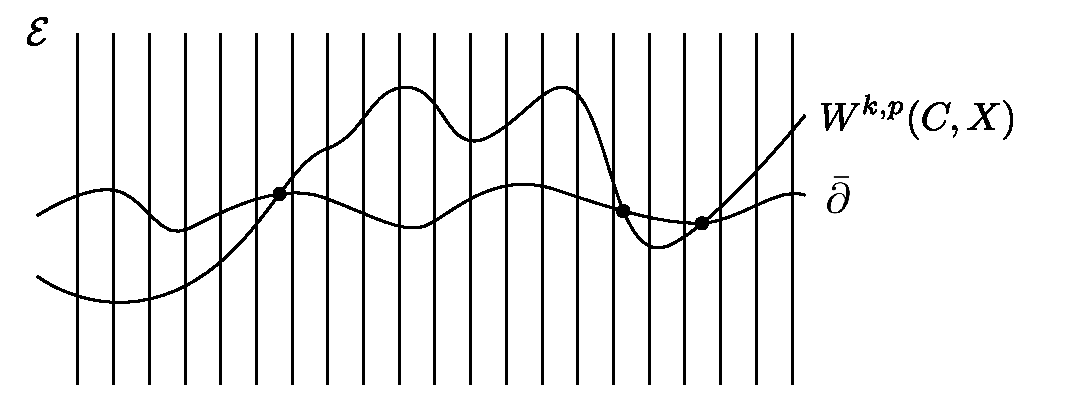
\includegraphics[width=0.8\textwidth]{sections_of_W.pdf}
\caption{The three intersection points pictured comprise
the moduli space:
$\cM\left( C , X \right) = 
\left\{ u: C\fromto X \st \left( du \right)^{0,1} = 0\right\}$
}
\label{fig:sections_of_W}
\end{figure}

The conclusion of this discussion, is that if
$D\barr{\p}$ is surjective at some point $p\in \cM\left( C , X \right)$, 
that is, some holomorphic map $u:C\fromto X$, 
then $\cM\left( C , X \right)$ is a smooth (Banach) manifold near $p$.

At $u:C\fromto X$, 
\begin{equation}
D_u \barr{\p}:
W^{k,p}\left( C , u^* TX \right)\fromto 
W^{k-1 , p}\left( C , \barr{\Hom}_\CC\left( TC , u^* TX \right) \right)
\end{equation}
measures the failure of $\exp_u \xi$ to be $\CC$-linear for small $\xi$.

\begin{defn}
Suppose we have two Banach spaces $X$ and $Y$.
Then an operator $A:X\fromto Y$ is called \emph{Fredholm} iff
$\ker A$ is finite dimensional, $\im A$ is closed and $\coker A$ is finite dimensional.
\end{defn}

\begin{thm}
Any elliptic operator of order $d$ on a compact manifold $M$ is Fredholm from
$W^{k,p}$ to $W^{k-d , p}$, in particular $D_u \barr{\p}$.
\end{thm}

In other words we can strike out the word Banach above, and write that
if $D\barr{\p}$ is surjective at some point $p\in \cM\left( C , X \right)$, 
then $\cM\left( C , X \right)$ is a smooth manifold near $p$.

We define the index of the operator to be
\begin{equation}
\ind\left( A \right) \ceqq \dim\left( \ker A \right) - \dim\left( \coker A \right)
\end{equation}
There ar emany ways to calculate, such as the Atiyah-Singer index theorem, 
but on Riemann surfaces we don't need such a poweful statemt.
We simply offer the result:
\begin{equation}
\ind\left( D_i \barr{\p} \right) = 
\left( 1 - g \right)\dim X+ \lr{2c_1\left( TX \right) , u_*\left[ C \right]}
\end{equation}
So this gives the dimension of the moduli space of curves.

\subsection{Generic transversality}

We now introduce a new space $\cJ$ of almost complex structures on $X$.
For example, we might take this to consist of the almost complex structures on $X$
of class $W^{k,p}$, so this would be some Banach manifold.

We can just cross everything from before with $\cJ$ to get:
\begin{equation}
\begin{cd}
\cE\times \cJ \arrow{d}\\
W^{k,p}\left( C , X \right) \times \cJ\arrow[bend right]{u}
\end{cd}
\end{equation}
where the sections just map $\left( u,J \right) \mapsto \left( \barr{\p}_J u , J \right)$.

Before, the zero set was just $\cM\left( C , X \right)$, and now
the zero set is
\begin{equation}
\cM\left( C , X , \cJ \right) \ceqq
\left\{ J\in \cJ , u: C\fromto X \st
u \text{ is } J \text{ holomorphic }\right\}
\end{equation}
Now we simply have $\pi: \cM\left( C , X , \cJ \right) \fromto \cJ$, 
where $\pi^{-1}\left( \left\{ J \right\} \right) = \cM\left( C , X , J \right)$.
Now it's much easier for the derivative to be surjective, since we have enlarged the base.
Now $\cM\left( C , X , \cJ \right)$ is a Banach manifold at $\left( u , J \right)$ iff
the following is surjective:
\begin{equation}
W^{k,p}\left( C , u^* TX \right)\dsum T_J \cJ
\fromto W^{k-1 , p}\left( C , \barr{\Hom}_\CC\left( TC , u^* TX \right) \right)
\end{equation}
Explicit calculation can show that this is surjective if $u$ is \emph{somewhere injective}
on every component of $C$.

\begin{thm}[Sard-Smale]
\label{thm:sard_smale}
The regular values of $\pi$ are of second Baire category.
That is, a countable intersection of open dense subsets.
In particular, it is dense.
\end{thm}

Of course the whole total space being smooth doesn't mean every fiber is smooth, but
the complement of the nonregular points is at least dense. 

\section{Topologies on moduli spaces and compactness}

We can impose many regularity conditions on the maps in $\cM\left( C , X \right)$,
and similarly, we can put many different topologies on this. 
A very strong topology is the $\cC^\infty$ topology where all derivatives would have to converge, 
on the other hand, the $\cC^0$ topology is very weak. 
However, regularity tells us that these topologies are the same.

\begin{proof}[Sketch proof]
Suppose $u_i$ converges to $u$ in $\cC^0$.
The derivatives might however exhibit bad behaviour.
Luckily, elliptic estimates imply that $\norm{u_i}_{\cC^k}$ is bounded.
Given this boundedness, Arzel\'a-Ascoli implies that there is a subsequence $u_{i_k}$
which is $\cC^\infty$ convergent to something, but it's already
$\cC^0$ convergent to $u$, so it must be $\cC^\infty$ convergent to $u$,
which means the whole sequence has to converge to $u$ in $\cC^\infty$.
\end{proof}

Let's talk about a moduli space without a fixed domain.
Define $\barr{\cM}_g\left( X \right)$ to consist of the pairs
$\left( C , u \right)$ such that $C$ is a nodal Riemann surface of genus $g$, 
and $u:C\fromto C$ holomorphic such that 
$\left\{ \phi : C\fromto C \st u\comp \phi = u \right\}$ is finite.
When this is the case, $u$ is said to be \emph{stable.}.

\begin{exm}
Nodal Riemann surfaces of genus $1$ of course consist of the smooth
Riemann surfaces of genus $1$, but also when we attach additional
copies of Riemann spheres as in \cref{fig:nodal_riemann}.
\begin{figure}
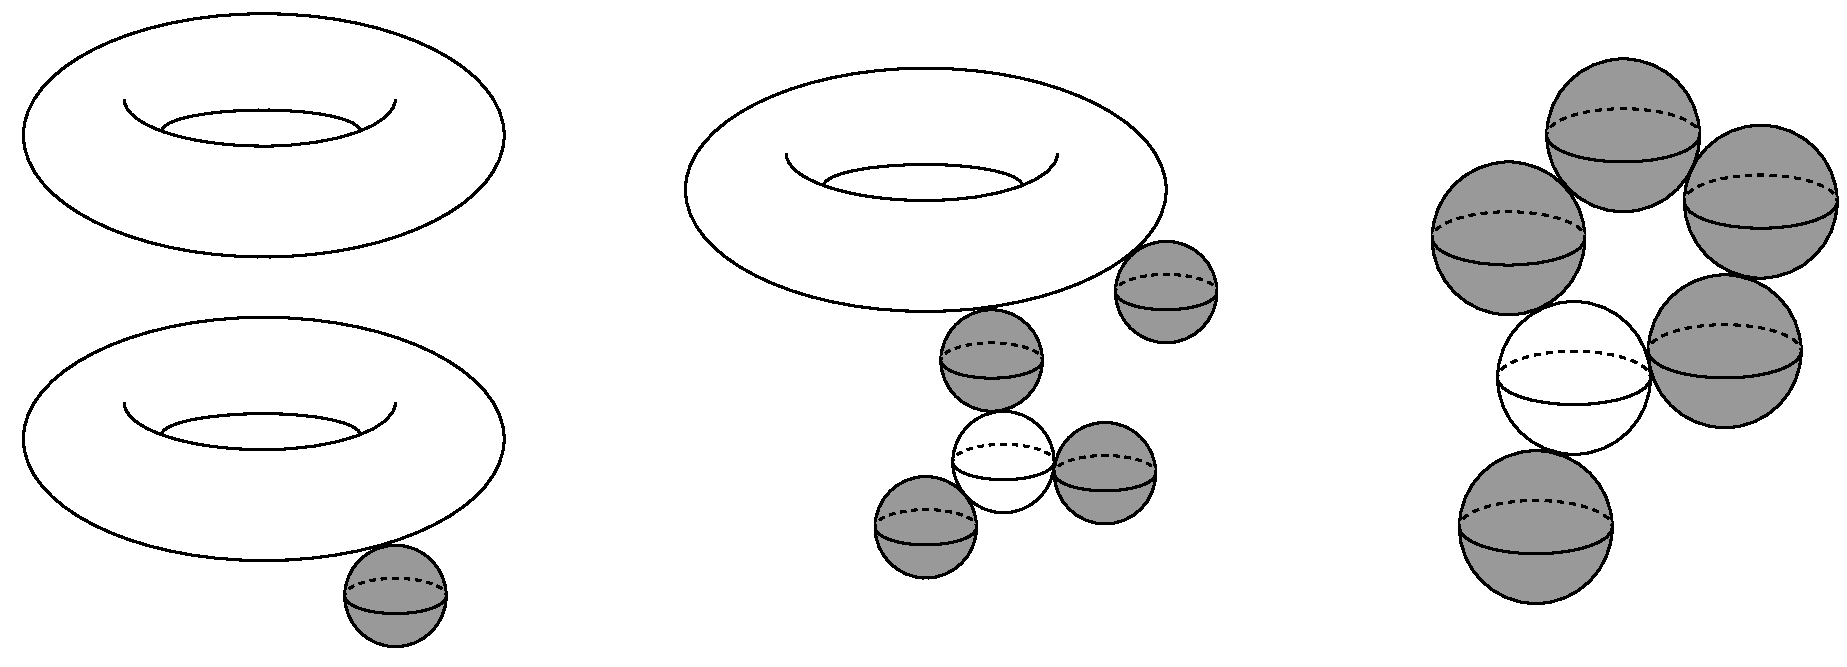
\includegraphics[width=\textwidth]{nodal_riemann.pdf}
\caption{Several examples of nodal Riemann surfaces. 
This is a classical Riemann surface, only now we allow for nodes. 
Note that the spheres colored gray are the regions where we insist on map 
$u$ be non-constant for reasons related to stability.}
\label{fig:nodal_riemann}
\end{figure}
\end{exm}

Consider some map from a surface with many nodes. 
By taking a resolution where we remove a node, and then glue a cylinder to the 
circular boundaries this creates, we can therefore get an induced map on
a surface with fewer nodes.
This motivates the following.
A neighborhood of $u:C\fromto X$ in $\barr{\cM}_g\left( X \right)$
consists of maps 
$u':C'\fromto X$ where $C'$ is a $\e$-small resolution of $C$, with $\e$-close
acs, and $u'$ is $\e$-close to $u$ in $\cC^0$.

Why is this stability condition from above required for this moduli space to make sense?
To see this, we consider the example in \cref{fig:nodal_riemann}.
Consider some curve $u$ defined on the top left surface.
Now consider the bottom left surface.
If we don't insist on stability, and allow for the map to be constant
on the attached Riemann sphere, then if we take the curve $u$, 
and just extend it to be a constant on the sphere, we get a curve $u'$
defined on the bottom left surface such that $u$ and $u'$ are actually regarded as different
curves.
But now, for any such unstable map, we can always just take a resolution
to get the stabilization, so our moduli space isn't Hausdorff.
However, as long as we insist on stability we have the following:

\begin{lem}
$\barr{M}_g\left( X \right)$ is Hausdorff
\end{lem}

This topology is called the Gromov topology.
In fact, we have:

\begin{thm}[Gromov]
$\barr{M}_g\left( X \right)$ is compact.
\end{thm}

\section{Symplectomorphism group of $S^2\times S^2$, Reeb orbits on $S^3$}

We now consider
\begin{equation}
\Symp\left( S^2 \times S^2 , \om_0 \dsum\om_0 \right)
\end{equation}
That is, the symplectomorphisms of this space with two factors having the same area.
We will use holomorphic curves to determine homotopy type of this group. 
We will first work to understand holomorphic curves with respect to the acs
$J_\splitt = J_0\dsum J_0$.
So we want maps in classes $\left( 1,0 \right)$ and $\left( 0,1 \right)$ in
$H_2\left( S^2 \times S^2 \right) = \ZZ\dsum \ZZ$, with domain $\CP^1$, that is, with genus $0$.
The only such maps are $S^2 \times \pt$ and $\pt\times S^2$ in $S^2 \times S^2$.
This gives us the foliation in \cref{fig:double_foliation}.
\begin{figure}
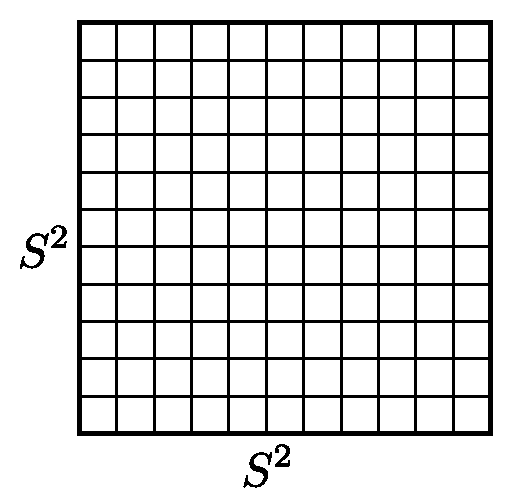
\includegraphics[width=0.3\textwidth]{double_foliation.pdf}
\label{fig:double_foliation}
\end{figure}

Let's think about transversality for a holomorphic immersion
$u: C\fromto X$. 
So we have our linearized operator 
$D:W^{k,p}\left( C , u^* TX \right) \fromto
W^{k-1,p}\left( C , \barr{\Hom}_\CC\left( TC , u^* TX \right) \right)$
which always fits into the following sequence with exact columns:
\begin{equation}
\begin{cd}
0\arrow{d} & 0\arrow{d}\\
W^{k,p}\left( C , TC \right) \arrow{d} \arrow{r}{D^T}&
W^{k-1 , p}\left( C , \barr{\Hom}_\CC\left( TC , TC \right) \right)\arrow{d}\\
W^{k,p}\left( C , u^* TX \right)\arrow{r}{D}\arrow{d}&
W^{k-1 , p}\left( C , \barr{\Hom}_\CC\left( TC , u^* TX \right) \right) \arrow{d}\\
W^{k,p}\left( C , u^* TX / TC \right)\arrow{r}{D^N}\arrow{d}&
W^{k-1 , p}\left( C , \barr{\Hom}_\CC\left( TC , u^* TX / TC \right) \right)\arrow{d}\\
0 & 0
\end{cd}
\end{equation}
where the rows are short exact sequences, and 
we are just taking the quotient.
Then we get the following exact sequence:
\begin{equation*}
0\fromto \ker D^T \fromto \ker D\fromto \ker D^N \fromto \coker D^T \fromto \coker D
\fromto \coker D^N \fromto 0
\end{equation*}
Note that $\ker D$ is the tangent space to $\cM\left( C , X \right)$, and
$\ker D^N$ is the tangent space of holomorphic maps to $X$ in the same topological type of $C$.

We should think of $D^T$ as controlling deformations of holomorphic structure on $C$
\begin{equation}
\ker D^T = H^0\left( C , TC \right)
\end{equation}
since this consists of the infinitesimal automorphisms of $C$ and
\begin{equation}
\coker D^T = H^1\left( C , TC \right)
\end{equation}
are the infinitesimal deformations of acs on $C$.

Let $u:C\fromto X$ be one of these curves $\pt \times S^2$
or $D^2 \times \pt$. Then 
\begin{equation}
D^N:
W^{k,p}\left( C , u^* TX / TC \right) \fromto
W^{k-1,p}\left( C , \barr{\Hom}_\CC\left( TC , u^*TX/TC \right) \right)
\end{equation}
is the Cauchy-Riemann operator on this bundle.
But $u^* TX / TC = \cO_{\CP^1}$ is just the trivial bundle for $C = \CP^1$,
so 
\begin{align}
\ker D^N = H^0\left( \CP^1 , \cO \right) = \CC
&&
\coker D^N = H^1\left( \CP^1 , \cO \right) = 0
\end{align}
The $\coker$ vanishing means the moduli spaces are transverse.

We now consider an arbitrary compatible $J$ on $S^2 \times S^2$. 
Suppose we have $u:\CP^2 \fromto \left( S^2 \times S^2 , J \right)$, 
in the class $\left( 1,0 \right)$ or $\left( 0,1 \right)$.
Since we're on $S^2 \times S^2$, the map
$\pi_2\left( S^2, S^2 \right)\lfromto{\sim} H_2\left( S^2 \times S^2 \right)$ is an isomorphism,
Therefore
\begin{equation}
u^*\left( T\left( S^2 \times S^2 \right) \right)
= TS^2 \dsum \CC
\end{equation}
as complex vector bundles.

If $u$ is a self transverse immersion,
$u:\CP^1 \tvi S^2 \times S^2$, then the number of double points satisfies
\begin{equation}
c_1\left( N_u \right) + 2 \#\left( \text{double points} \right) = 
\left( u_*\left[ \CP^1 \right]  \right)\inter \left( u_*\left[ \CP^1 \right] \right)
\end{equation}
Since $u$ is an immersion, 
$u^*\left( T\left( S^2 \times S^2 \right) \right) = TS^2 \dsum N_u$.
Now we have:
\begin{align}
c_1\left( TS^2 \dsum N_u \right) = c_1\left( TS^2 \right) + c_1\left( N_u \right) &=
c_1\left( u^*\left( T\left( S^2 \times S^2 \right) \right) \right) \\
&= c_1\left( TS^2 \right) + c_1\left( \CC \right)
\end{align}
so $c_1\left( N_u \right) = c_1\left( \CC \right)$, and since
complex line bundles over $S^2$ are classified by the first Chern class, we get
$N_u \simeqq \CC$.
This all means that $u$ is an embedding.

For general $J$-holomorphic $u: \CP^1 \fromto S^2 \times S^2$ in class
$\left( 1,0 \right)$ or $\left( 0,1 \right)$, 
$u$ is an embedding (and immersed).
Hence, $\ker D^N = \CC$
and $\coker D^N = 0$, as previously.
In particular, $u$ is transverse.

Recall $\cM_{0,0}^{1,0}$ consists of the
genus $0$ $J$-holomorphic curves in $S^2 \times S^2$ in class
$\left( 1,0 \right)\in H_2\left( S^2 \times S^2 \right)$.
Since $u$ is transverse we have that
$\cM_{0,0}^{1,0}\left( S^2 \times S^2 , J \right)$ and
$\cM_{0,0}^{0,1}\left( S^2 \times S^2 , J \right)$ are cut-out
transversely for every compatible acs $J$.
This is a miracle that happens only in dimension $4$.

For any $J$, there exists a path $J_t$ from
$J = J_0$ to $J_1 = J_\splitt$.
Then we look at the parameterized moduli space
\begin{equation}
\begin{cd}
\cM_{0,0}^{1,0}\left( S^2 \times S^2 , \left\{ J_t \right\}_{t\in \left[ 0,1 \right]} \right)
\arrow{d}{\pi}\\
\left[ 0,1 \right]
\end{cd}
\end{equation}
where $\pi$ is proper by Gromov compactness.

Define the energy to be the value given by
\begin{equation}
\int_\om: H_2\left( S^2 \times S^2 \right) \fromto \RR
\end{equation}
Since the two factors have the same area, $\left( 1,0 \right)$
and $\left( 0,1 \right)$ have the minimal positive value of $\int \om$.
Note that if $u:C\fromto C$ is $J$-holomorphic and non-constant, then
$\in_C u^* \om > 0$, 
which is precisely the definition of $J$ being tamed by $\om$. 

In addition to being proper, $\pi$ is also a submersion.
This is just the statement that all fibers cut out transversely.
But we know the fiber $\pi^{-1}\left( J_\splitt \right) = S^2$, 
which means $\pi^{-1}\left( J \right) = S^2$.
Thus for any compatible $J$, the $J$-holomorphic curves in classes
$\left( 1,0 \right)$ and $\left( 0,1 \right)$ from a pair of $\trans$ foliations.
Even with respect to a strange acs, such as in \cref{fig:strange_acs}, 
we get a foliation by these spheres.
\begin{figure}
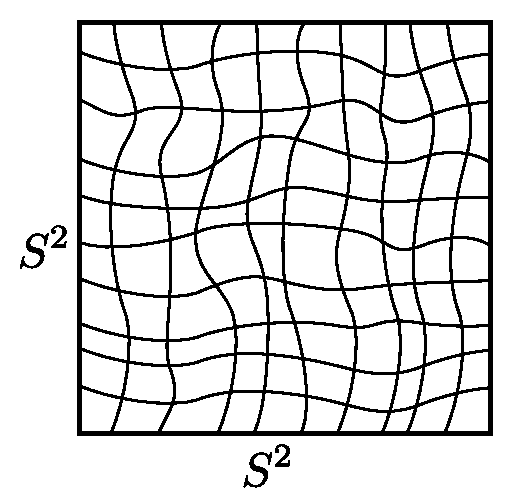
\includegraphics[width=0.4\textwidth]{warped_foliation.pdf}
\caption{For arbitrary acs $J$, we get this same well-behaved foliation by spheres,
only now it might exhibit nonstandard behaviour.}
\label{fig:strange_acs}
\end{figure}
The spheres are disjoint because of 
positivity of the intersection.

Finally, we consider the actual group of symplectomorphisms of
$S^2 \times S^2$.
Consider the classifying space:
\begin{equation}
B\Symp\left( S^2 \times S^2 , \om_0 \dsum \om_0 \right)
\left\{  \left( V, \om \right) \st \exists
\left( v, \om \right) \simeqq \left( S^2 \times S^2 , \om_0 \dsum \om_0 \right)\right\}
\end{equation}
Think of this as a set of submanifolds of $\RR^\infty$. 
So given a symplectic manifold, we can always consider the collection of compatible almost
complex structures, which
is contractible. So the forgetful map:
\begin{equation}
\left\{  \left( V, \om , J\right) \st \exists
\left( v, \om \right) \simeqq \left( S^2 \times S^2 , \om_0 \dsum \om_0 \right), J\text{ compatible }\right\}
\fromto B\Symp\left( S^2 \times S^2 , \om_0\dsum \om_0 \right)
\end{equation}
has contractible fibers, so this is a homotopy equivalence.

\begin{rmk}
These classes $\left( 1,0 \right)$ and $\left( 0,1 \right)$ 
are precisely the classes in $H_2$ of minimal positive energy and zero 
self intersection.
\end{rmk}

Given $\left( V , \om , J \right)$ in the above set, we get
two transverse foliations by $J$-holomorphic copies of $S^2$
in the classes $\left( 1,0 \right)$ and $\left( 0,1 \right)$.

Now consider the set
\begin{equation}
\left\{ \left( V , \om , J , \om' \right) \st \left( v,\om \right) \simeqq
\left( S^2 \times S^2 , \om_0 \dsum \om_0 \right) , J\text{ compatible},
\om' \text{ split wrt} J\right\}
\end{equation}
This condition on $\om'$ is equivalent to $\om'$ being a sum of an 
area form of total area $1$, on leaf space of foliation $i$.
Now we can again map this to the set of triples $\left( V , \om , J \right)$,
and the fibers will again be contractible, so this is again a homotopy equivalence.
Now consider the following facts:
\begin{fact}
\item Note $J$ is compatible with $\om'$, because at each point
we can decompose the tangent space with respect to he foliations, 
and both $J$ and $\om'$ are split with respect to this decomposition.
\item $\om$ and $\om'$ are cohomologous.
\end{fact}
Together, using Moser's theorem,
these imply that 
$\left( V , \om \right)$ and $\left( V , \om' \right)$
are in fact symplectomorphic.

Therefore this set is the same as:
\begin{equation}
\left\{ \left( V , \om , J , \om' \right)\st
\left( V' , \om' \right) \simeqq \left( S^2 \times S^2 , \om_0 \dsum \om_0 \right)
J \text{ compatible with } \om,
\om'\text{ split wrt }J\right\}
\end{equation}
now we can map this to the set
\begin{equation}
\left\{ \left( V , \om' , J \right) \st
\left( V , \om' \right)\simeqq \left( S^2 \times s^2 , \om_0 \dsum \om_0 \right) , 
J\text{compatible with } \om' , 
\om' \text{ split wrt J }\right\}
\end{equation}
which is an equivalence. 
Finally, we can deformation retract this to
\begin{equation}
\left\{ \left( V , \om' , J \right) \st
\text{ same conditions, except require leaves have same acs.}\right\}
\end{equation}
and this is also an equivalence. But this is the same as
\begin{equation}
\left\{ \left( V, \om' , J \right) \st
\left( V , \om' , J \right) \simeqq
\left( S^2 \times S^2, \om_0 \dsum \om_0 , j_0 \dsum j_0 \right)\right\}
\end{equation}
so we have:
\begin{equation}
B\Aut\left( S^2 \times S^2 , \om_0 \dsum \om_0 , j_0 \dsum j_0\right)
= \left( \SO\left( 3 \right) \times \SO\left( 3 \right) \right)\rtimes \ZZ / 2
\end{equation}

By similar methods, we can show:

\begin{thm}
$\Symp\left( \CP^2 , \om_\std \right)$ is homotopy equivalent to
$\PU\left( 3 \right) \simeqq \PGL_3\CC$.
\end{thm}

\begin{prop}
For any compatible $J$ on $\CP^2$ and $p,q\in \CP^2$, 
there exists a unique pseudo-holomorphic $\CP^1 \fromto \CP^2$ of degree $1$ through $p$, $q$
\end{prop}

If we take some $S^3 \subeq \CC^2$, this carries what is called a contact structure
$\xi\subeq TS^3$, where
$\xi \ceqq TS^3 \cap J\left( TS^3 \right)$.
For a $1$-form $\al$ on $S^3$ with $\ker \al= \xi$, 
we can define a vector field $R_\al$ on $S^3$ by
$\al\left( R_\al \right) = 1$ and $d_\al\left( R_\al , \cdot \right) = 0$.

\begin{cor}
Any Reeb vector field $R_\al$ for the standard contact structure $\xi$
on $S^3$ has a closed orbit. 
\end{cor}

\begin{proof}
Consider $\CP^2$ with $\CC^2$ inside it. 
Contact forms on $S^3$ correspond to star-shaped regions in $\CC^2$
as in \cref{fig:star_shaped}.
\begin{figure}
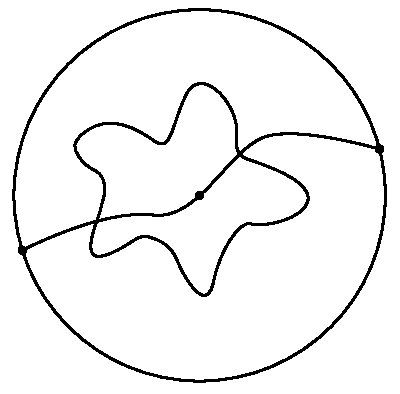
\includegraphics[width=0.4\textwidth]{star_shaped.pdf}
\caption{Some star-shaped region in $\CC^2$ which corresponds to
a contact form on $S^3$.}
\label{fig:star_shaped}
\end{figure}
Then we perform a neck-stretch degeneration of $J$ along this hypersurface corresponding
to $\al$ and holomorphic curves in the neck region converge to cylinders over Reeb orbits.
\end{proof}

\section{Examples of bubbling}

Consider some maps $u_n$ from a Riemann surface to $X$. 
Recall that, to this, we can associate the energy
\begin{equation}
E\left( u_n \right) = \int u_n^* \om =
\int \abs{d u_n}^2
\end{equation}
The point is, the RHS is useful for analysis, but the middle is more easily computable.
In particular, if these maps are in the same homology class, then these have the same energy.
Bubbling occurs when energy concentrates around some point.
This is intuitively clear, because energy is really just area, so a large amount of
area is trapped in this sort of localized space.
Gromov compactness tells us that when $u_n$ does not admit a convergent subsequence, then
we have to have this sort of bubbling phenomenon.
We now consider some concrete example to illustrate how this isn't
just some sort of analytic annoyance, but rather a geometric phenomenon.

Recall the blowup construction.
In general, we can take any complex manifold $X$ of complex dimension $2$ and $x\in X$, and define
the blowup:
\begin{equation}
\Bl_x X = \tilde X = X\minus \left\{ x \right\}\un \PP\left( T_x X \right)
\end{equation}
This is easy to write as a set, but we have to work a bit harder for the topology.
Consider $\CC^2$ with the origin regarded as our point $x$.
Then at the origin we put a copy of $\PP^1$ in here, so all of the
lines which cross at the origin now cross this line at different points. 
The picture to image here is as in \cref{fig:blowup}.
\begin{figure}
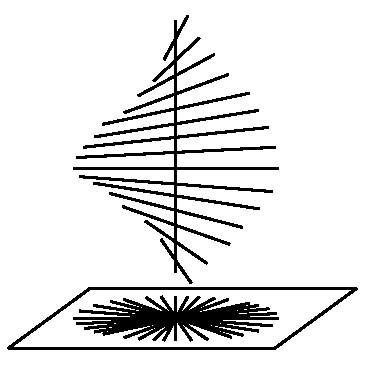
\includegraphics[width=0.4\textwidth]{blowup.pdf}
\caption{The blowup of $\CP^2$.}
\label{fig:blowup}
\end{figure}
Explicitly:
\begin{equation}
\left\{ 
\left( \left( x,y \right) , \left[ X:Y \right] \right)\in \CC^2 \times \PP^1 \st
xY - yX = 0
\right\}=
\left\{ \left( p,l \right) \st p\in l \right\}
\end{equation}
then for a generic manifold we can just glue in this construction locally.

Now let $X$ be the blowup of $\CP^2$ at $\left( 0,0,1 \right)$. 
We know this projects to $\CP^2$.
Consider some line which comes close to the origin, but does not meet it. 
This is shown in red in \cref{fig:blowup_intersection}.
\begin{figure}
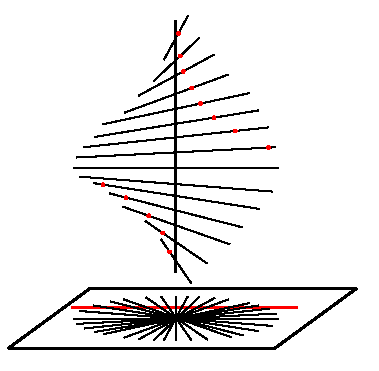
\includegraphics[width=0.8\textwidth]{blowup_intersection.pdf}
\caption{The red line comes close to the origin, but does not touch it. 
The intersections between the red line, and the lines going through the origin
in $\CP^2$, are plotted in red in the blowup.}
\label{fig:blowup_intersection}
\end{figure}
If the red line were to actually touch the boundary, it would be
exactly coinciding with one line through the origin, 
and only intersect all of the other lines at a single point. 
Therefore we see that this intersection, as viewed in the blowup,
gets an extremely large ``length'' as viewed in the picture, 
or in proper dimensions, a large area, and therefore energy. 
Explicitly, the domain gets closer and closer to being two spheres joined at a point.

As another example, consider the curve given by
$y^2 = x^2 \left( x + 1 \right)$ as in \cref{fig:elliptic_curve}.
We intersect the curve with the red line, and as we approach the node, 
when we lift to the blowup with the limiting behaviour on the right.
So again we see this bubbling phenomenon, since if the line were to actually pass through 
the node, it would not have this energy accumulation.

\begin{figure}
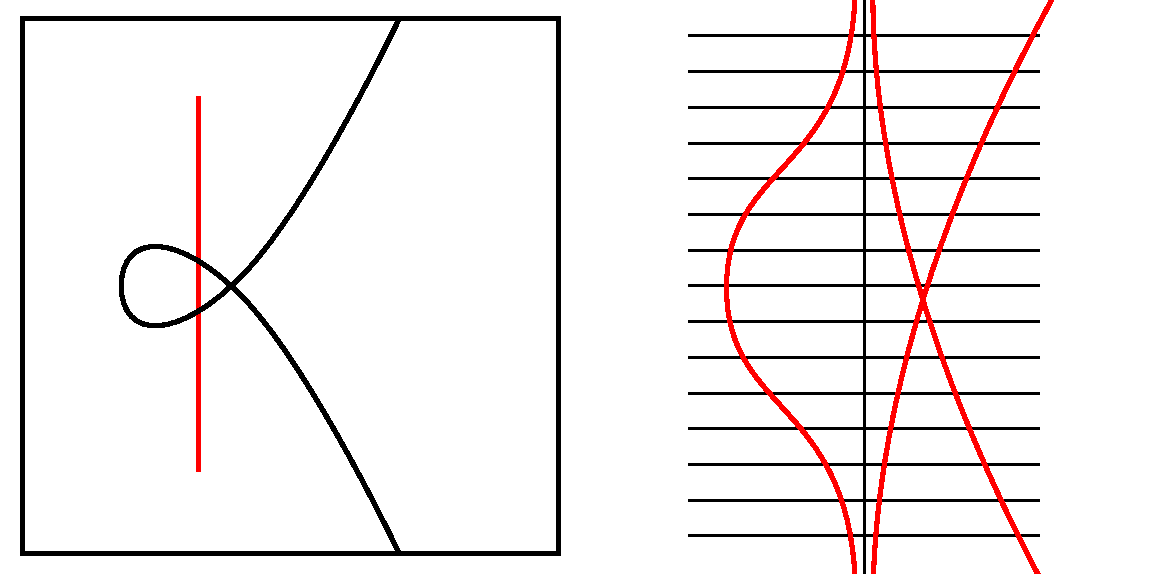
\includegraphics[width=0.8\textwidth]{elliptic_curve.pdf}
\caption{The elliptic curve $y^2 = x^2\left( x + 1 \right)$ is plotted, and
then we intersect the curve with the red line near, but not intersecting,
the node. We then lift this to the blowup on the right.}
\label{fig:elliptic_curve}
\end{figure}

The domain of this example approaches becoming three spheres joined
as in \cref{fig:mickey}.

\begin{figure}
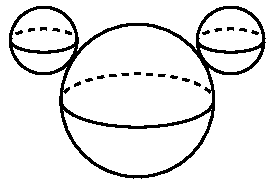
\includegraphics[width=0.3\textwidth]{mickey.pdf}
\caption{The domain of the elliptic curve example approaches having something like this
as its domain.}
\label{fig:mickey}
\end{figure}


\section{Fukaya categories}

So far we have regarded holomorphic-curves as geometric objects. 
Now we're going to forget some of these things and concern ourselves more over
enumerative questions. 

\subsection{Construction of classical Fukaya category}

Fix a symplectic manifold $\left( X , \om \right)$, and assume it is exact.
So $\om = d\lam$ for some $1$-form $\lam$. 
This forces $X$ to be noncompact.\footnote{
This is because $\om^n$ is a volume form, and $\om = d\lam$,
so $\om^n = 0\in H^{2n}\left( X \right)$.}
Now consider exact Lagrangians $L$.
This means in addition to $\restr{\om}{L}= 0$,
we also have $\restr{\lam}{L} = df$ for some $f$.

\begin{rmk}
One reason for $\om$ to be exact, is to get control over the moduli spaces.
Suppose the manifold contains a bunch of holomorphic spheres.
If this was the case, then we could just glue in some extra sphere to any disk, and we would get
a disk of higher energy.
Then we could do this for an $n$-fold cover of the sphere, and we would get disks of arbitrary
energy.
But when it's exact, we have no holomorphic spheres.

Exactness also helps achieve transversality.
It rules out bubbling holomorphic spheres which are hard to make transverse.
\end{rmk}

\begin{defn}
The Fukaya category $\cF\left( X , \lam \right)$ has objects exact
Lagrangians, and morphism spaces are 
\begin{equation}
\CF^*\left( L , K \right) \ceqq
\bdsum_{p\in L\cap K} \ZZ / 2\ZZ
\end{equation}
for any two exact Lagrangians $L_0$ and $L_1$.
\end{defn}

Recall that the Floer complex $\CF^*$ is equipped with a differential
\begin{equation}
d: \CF^*\left( L , K \right) \fromto \CF^*\left( L , K \right)
\end{equation}
where $p$ maps to the count
\begin{equation}
p\mapsto
\sum_q \# \cM\left( D \right) q
\end{equation}
where the disks $D$ are as in the first disk in \cref{fig:disks}.
Note that $\cM$ has dimension $\ind\left( q \right) - \ind\left( p \right) - 1$, 
and $\# \cM$ is the count of elements in case $\dim M = 0$.
Also note that $\cM$ is the moduli space of disks up to reparameterization.

\begin{figure}
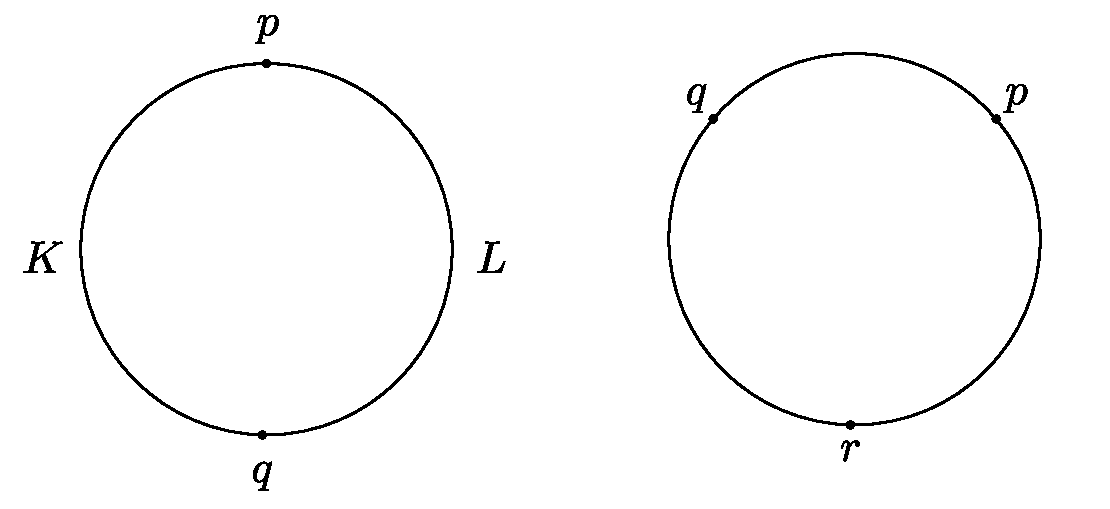
\includegraphics[width=0.5\textwidth]{disks.pdf}
\caption{(Left) Disk with two punctures which are summed over in the 
differential on the Floer complex.
(Right) Disk with three punctures which are summed over in the ``composition'' map
on the Floer complex.}
\label{fig:disks}
\end{figure}

Now we want to define a sort of composition 
\begin{equation}
\mu^2: \CF^*\left( L_0 , L_1 \right) \tp \CF^*\left( L_1 , L_2 \right) \fromto
\CF^*\left( L_0 , L_2 \right)
\end{equation}
where we explicitly map:
\begin{equation}
p\tp q \mapsto \sum_r \# \cM\left( D \right) r
\end{equation}
where $D$ denotes disk as in the right of \cref{fig:disks}.
Similarly, $d$ is sometimes denoted $\mu^1$.

But this isn't quite associative.
If we compose three morphisms:
\begin{equation}
\CF^*\left( L_0 , L_1 \right) \tp 
\CF^*\left( L_1 , L_2 \right) \tp 
\CF^*\left( L_2 , L_3 \right) 
\fromto \CF^*\left( L_0 , L_3 \right)
\end{equation}
we can send 
\begin{equation}
p\tp q \tp r \mapsto
\sum_s \# \cM\left( D \right)s
\end{equation}
but there is now some ambiguity in what disk we are counting. 
We might choose either one of the disks in \cref{fig:disks2}.
\begin{figure}
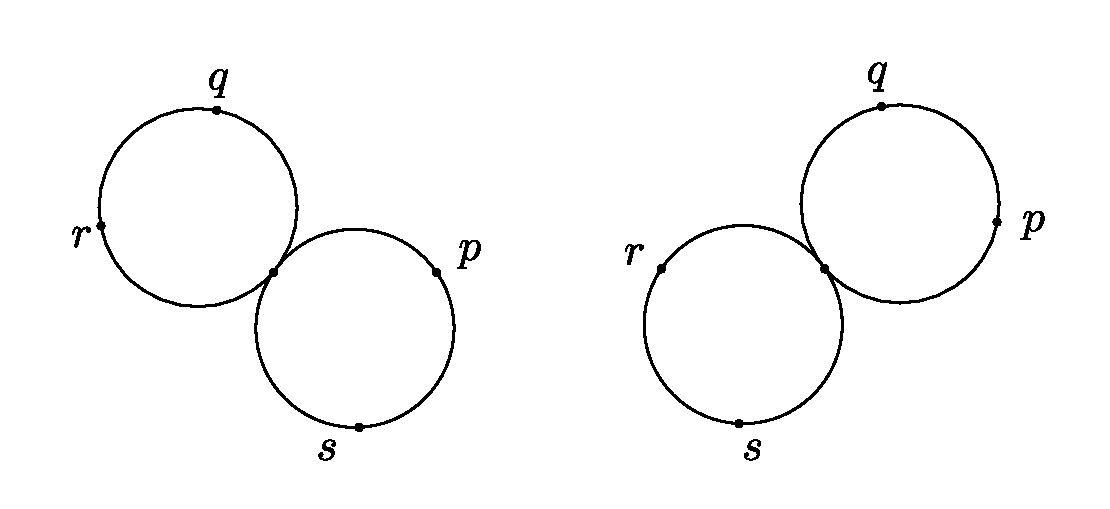
\includegraphics[width = 0.8\textwidth]{disks_2.pdf}
\caption{The two disks which we might count in our attempt at 
showing $\mu^2$ is associative.}
\label{fig:disks2}
\end{figure}

In order to relate these, we define another relation:
\begin{equation}
\mu^3:
\CF^*\left( L_0 , L_1 \right) \tp 
\CF^*\left( L_1 , L_2 \right) \tp 
\CF^*\left( L_2 , L_3 \right) 
\fromto \CF^*\left( L_0 , L_3 \right)
\end{equation}
which sends:
\begin{equation}
p\tp q \tp r \mapsto
\sum_s \# \cM \left( D \right) s
\end{equation}
where the disks $D$ are as in \cref{fig:disks3}.
\begin{figure}
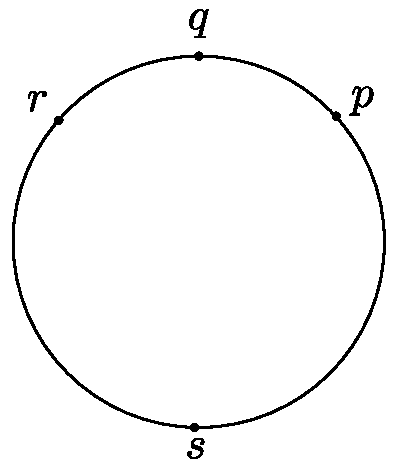
\includegraphics[width=0.3\textwidth]{disks_3.pdf}
\caption{$\mu_3$ sends $p\tp q \tp r$ to the count of
disks of this sort.}
\label{fig:disks3}
\end{figure}
\begin{fact}
$\mu^3$ is a chain homotopy between $\mu^2\left( \mu^2\left( \cdot , \cdot \right) , \cdot \right)$
and $\mu^2\left( \cdot , \mu^2\left( \cdot , \cdot \right) \right)$
\end{fact}

\subsection{Degeneration}

These disks with marked points (or punctures) we have
been discussing have so-called degenerations. 
These motivate some structure relations on $\CF$.
When we have two points on the boundary, we have that the disk can
degenerate to two disks intersecting at a point, with one marked point
on each. This gives us $d^2 = 0$.

Now with three points, we get degenerations as in
\cref{fig:degenerations}.

\begin{figure}
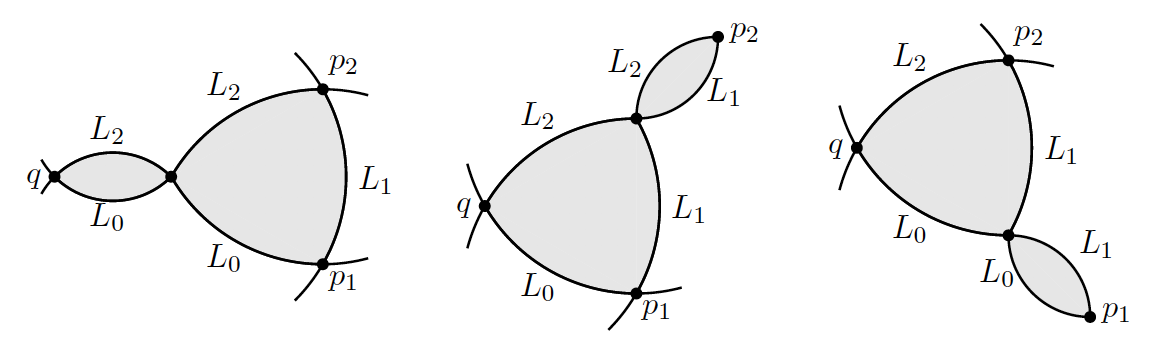
\includegraphics[width=0.8\textwidth]{degenerations.png}
\caption{The three potential degenerations of the disk with three punctures,
which give us the Leibniz rule for $\mu^1$ and $\mu^2$.}
\label{fig:degenerations}
\end{figure}

This gives us
\begin{equation}
\mu^2\left( \mu^1\left( \cdot  \right) , \cdot  \right) +
\mu^2\left( \cdot , \mu^1\left( \cdot \right) \right) + 
\mu^1\left( \mu^2\left( \cdot , \cdot \right) \right) = 0
\end{equation}
which is exactly the statement hat $\mu^2$ is a chain map.

\begin{exr}
Repeat this for the $\mu^3$ case.
\end{exr}

This isn't a category in the usual sense as we've seen it so far. 
In fact, it's an $\cA^\infty$ category,
so we also have higher homotopies, which tells us there's only one way to compose morphisms.
Generalizing the above, 
the Fukaya category has the higher operations 
\begin{equation}
\mu^k:\CF\left( L_0 , L_1 \right) \tp \cdots \tp \CF\left( L_{k-1} , L_k \right)
\fromto \CF\left( L_0 , L_k \right)\left[ 2-k \right]
\end{equation}
of degree $k\geq 1$ satisfying the $\cA_\infty$ relations, counting disks as in \cref{fig:general_disk}.

\begin{figure}
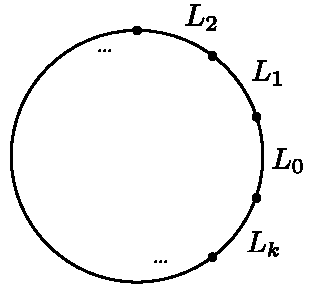
\includegraphics[width=0.3\textwidth]{general_disk.pdf}
\caption{The type of disk counted by $\mu^k$.}
\label{fig:general_disk}
\end{figure}

The conditions that these $\mu^k$ must satisfy can be written explicitly as:
\begin{equation}
\sum_{l=1}^j \sum_{j = 0}^{k-l}
\left( -1 \right)^* \mu^{j+1 -l}
\left( p_k , \cdots , p_{j + l + 1} , 
\mu^l\left( p_{j+l} , \cdots , p_{j+1} \right) , p_j , \cdots , p_1\right) = 0
\end{equation}
where $* = j + \deg\left( p_1 \right) + \cdots + \deg\left( p_j \right)$, 
though this if of course not of interest to us since we are working over $\ZZ / 2\ZZ$.
These can be understood as coming from summing over contributions from trees which
can also be viewed as degenerations of disks.
We consider the \emph{associahedron} $\barr{R}_{k,1}$
to a given $k\in \ZZ$.
This is the compactification of the space of potential conformal structures
with $k+1$ marked points. 
The top-dimensional facets correspond to nodal degenerations of a standard disk
$D$ to a union of disks, where each component has at least $2$ of
the $k$-marked points, and the higher codimension faces
correspond to nodal degenerations with more components. 
See \cref{fig:associahedron_1} for the example $k = 3$.

\begin{figure}
\centering
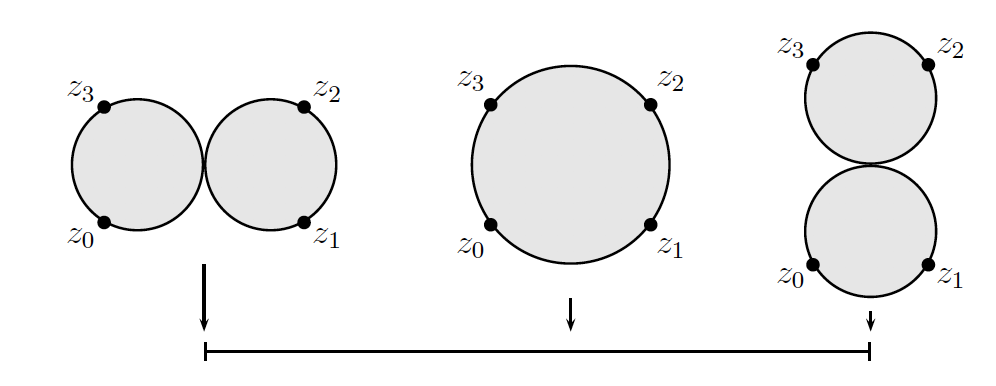
\includegraphics[width=0.7\textwidth]{associahedron_1.png}
\caption{The associahedron for $k = 3$.}
\label{fig:associahedron_1}
\end{figure}

\begin{rmk}
This is all sort of forced upon us.
If we consider how to count disks of some sort, 
then the conditions we will look for are exactly the 
conditions for an $\cA_\infty$ category.
\end{rmk}

\subsection{Wrapped Fukaya category}

If our exact symplectic manifold
$\left( X , \lam \right)$
is cylindrical at $\infty$, we can define the so-called
wrapped Fukaya category $\cW\left( X \right)$.
Cylindrical just means that near infinity, $X$ is isomorphic to
$\left( \RR_{s\geq 0}\times Y , e^s \al \right)$ for some contact form
$\al$ on $Y$.
Take the same objects as $\cF\left( X \right)$,
only now the morphisms are define by flowing the first
argument by the Reeb flow of $\al$, which happens to
also be the Hamiltonian vector field of $e^s$.
In other words, 
\begin{equation}
\CW^*\left( L , K \right) =
\Hom_{\cW\left( X \right)}\left( L, K \right) = 
\CF^*\left( \Phi L , K \right)
\end{equation}
where $\Phi$ is the flow of this vector field.

\begin{exm}
Consider the cylinder $X = \RR\times S^1 = T^* S^1$ as in the left of
\cref{fig:cylinder}.
\begin{equation}
\Hom_{\cW\left( T^* S^1 \right)} \left( K , K \right) = 
\HF^*\left( L , K \right) = \FF_2\left[ t , t^{-1} \right]
\end{equation}
Here we are effectively twisting for infinite time. 
If we were twisting a finite amount it would look like the right in \cref{fig:cylinder}.
\begin{figure}
\centering
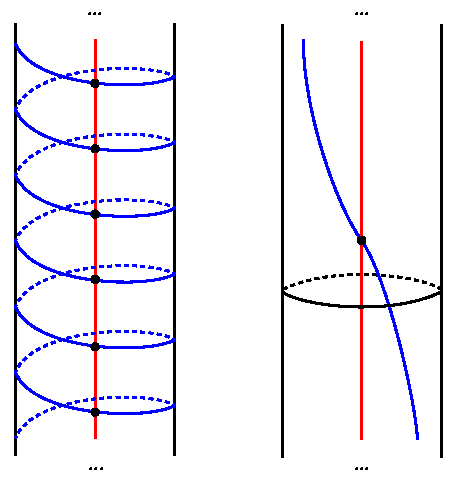
\includegraphics[width=0.6\textwidth]{cylinder.pdf}
\caption{(Left) The cylinder with with two exact Lagrangians
$K$ and $L$, one obtained by twisting the other at infinity.
(Right) The cylinder with an exact Lagrangian twisted
in a finite sense.}
\label{fig:cylinder}
\end{figure}
\end{exm}

Consider $\cM\left( T^* Q \right)$
where $T^* Q$ is exact, and cylindrical at $\infty$. 
If we choose a Riemannian metric on $Q$, we get a contact
form on $S^* Q$, whose Reeb flow is the geodesic flow.
This means that if we consider the wrapped Floer cochains, 
$\CW^*\left( T_p^* Q , T_q^* Q \right)$, as vector spaces this is the same as
$\FF_2\left[ \text{geodesics }p\leadsto q \right]$ as in \cref{fig:geodesic}.
\begin{figure}
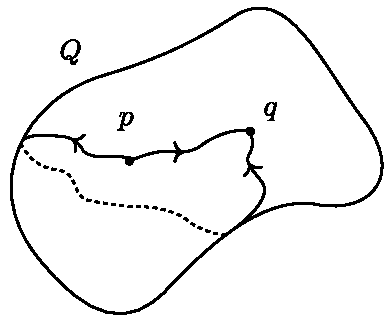
\includegraphics[width=0.5\textwidth]{geodesic.pdf}
\caption{Two geodesics both from $p$ to $q$ on $Q$.}
\label{fig:geodesic}
\end{figure}

\begin{thm}[Abbondandolo-Schwarz]
\begin{align}
\HW^*\left( T^*_p Q , T_q^* Q \right) &= H_{-*}\left( \Om_{p,q} Q \right) 
\\&=H_{-*}\left( \left\{ \gamma:\left[ 0,1 \right] \fromto Q \st \gamma\left( 0 \right) = p, 
\gamma\left( 1 \right) = q\right\} \right)
\end{align}
\end{thm}

\begin{rmk}
Another description of the map 
$\Hom_{-*}\left( \Om_{p,q} Q \right)\fromto
\HW^*\left( T_p^* Q , T_q^* Q \right)$ is as follows.
Suppose we have $Q$ and two points $p$ and $q$.
If these points are sufficiently close, there is a 
canonical shortest path, which corresponds to a cycle
since the differential can only decrease the length.
Now decide to only care about these short ones. 

\begin{figure}
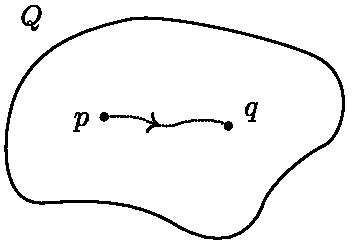
\includegraphics[width=0.6\textwidth]{discrete_geodesic.pdf}
\caption{We can discretize this geodesic, so all of the adjacent points
are ``close enough'' to find a canonical path between them.}
\label{fig:discrete_geodesic}
\end{figure}
Now take any path from $p$ to $q$, and discretize as in
\cref{fig:discrete_geodesic}.
Each discrete point and its adjacent neighbor has a relevant path, 
but the composition at large may not be one we care about, so
this isn't really a category.

Now consider the category $\cat{C}$ whose objects are the fibers
$T_p^* Q$ and whose morphisms are
``freely generated'' by the unique short geodesics between pairs of close by points.

There is a tautological functor from $\cC$ to $\cW\left( T^* Q \right)$. 
\begin{clm}
$\Hom_\cC\left( T^*_p Q , T^*_q Q \right) = C_{-*}\left( \Om_{p,q}Q \right)$
\end{clm}
\end{rmk}

\begin{thm}[Abouzaid]
The objects
$T_q^* Q\in \cW\left( T^* Q \right)$ generate $\cW\left( T^* Q \right)$
\end{thm}

\subsection{Arnold's conjecture}

\begin{con}[Arnold]
For any exact compact Lagrangian $L\subeq T^* Q$, 
$L$ is isotopic to the zero section.
\end{con}

\begin{figure}
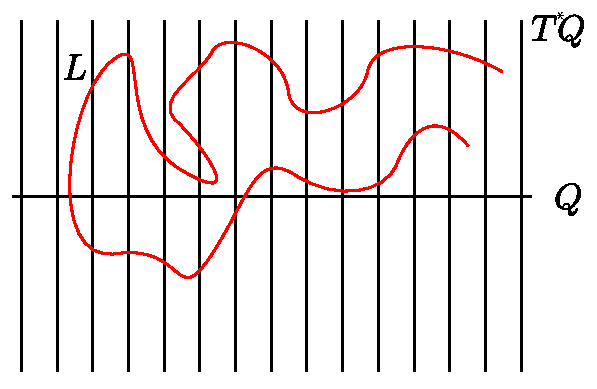
\includegraphics[width=0.5\textwidth]{arnold.pdf}
\caption{We have some Lagrangian $L$ in $T^*Q$, and
we want to see what happens when we project this down to $Q$.}
\end{figure}
The picture here is as in 
and then the projection of $L$ down to $Q$ is a
simple homotopy equivalence
This is trivial for $Q = S^1$, 
and this is known for $Q = S^2$
and $Q = \RP^2$.

\begin{thm}[Fukaya-Seidel-Smith-Nadler-Zaslow-Abouzaid]
$L\subeq T^* Q$ compact exact, then $L\fromto Q$ is a simple homotopy
equivalence.
\end{thm}

We will prove a weaker version of this.
First we need:

\begin{thm}[Weinstein]
A neighborhood of $L$ is symplectomorphic to 
a neighborhood of the zero section in $T^* L$.
\label{thm:weinstein_neighborhood}
\end{thm}

\begin{prop}[Floer]
If $L\subeq X$ is exact, then
$\HF^*\left( L , L \right) = H^*\left( L \right)$.
\end{prop}

\begin{proof}
\begin{figure}
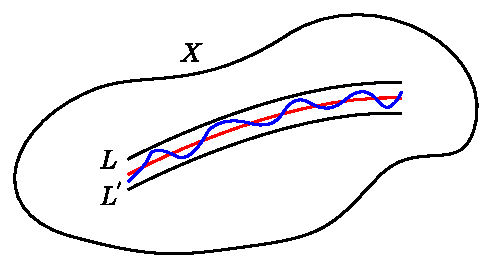
\includegraphics[width=0.7\textwidth]{perturbation.pdf}
\caption{We take an exact Lagrangian $L$ in $X$, and a tubular neighborhood surrounding it. 
Then we perturb $L$ to get another exact Lagrangians $L'$ in $X$.}
\label{fig:perturbation}
\end{figure}
We have the Weinstein neighborhood \cref{thm:weinstein_neighborhood}
which gives us a canonical tubular neighborhood of such an $L$ as in
\cref{fig:perturbation}.
Now to compute this, we need to perturb $L$ slightly. 
Consider the Hamiltonian perturbation $L'$ of $L$ given inside $T^*L$ by the graph
of $df$ for some Morse function $f:L\fromto \RR$, as in \cref{fig:perturbation}.

Now the intersections of $L'$ and $L$ are the zeros of $df$, 
so they are also critical points of $f$, so 
\begin{equation}
\CF^*\left( L' , L \right) = \CM^*\left( L , f \right)
\end{equation}
as abelian groups, where $\CM^*$ denotes the Morse complex.
Moreover, for appropriate choice of acs $J$, 
the differentials are actually the same.

Exactness is necessary, because
these disks of small energy are identified with the Morse trajectories. 
We might also have big disks which goes out through the entire manifold, 
and the exactness rules them out.
This is because for a disk $u$,
\begin{equation}
E\left( u \right)= \int _{D^2} u^* \om = \int_{D^2} u^* \left( d\lam \right)
= \int_{\p D^2} u^* \lam = 0
\end{equation}
and the boundary is contained in $L$, where $\lam$ is just $df$, so this is $0$.
\end{proof}

Now we return to the conjecture.
We have the following hypotheses:
$Q$ is simply connected, and Whitney class $w_2 = 0$.
$L\subeq T^* Q$ is compact, exact, and has Maslov class $0$. 
Given $L$, we can associate a local system $\cE_L$ on $Q$
whose fiber over $q\in Q$ is 
$\CW^*\left( T_q^* Q , L \right)$, which we notice is finite dimensional,
since $L$ is compact.

The fact that the cotangent fibers $T^*_q Q$
generate the Fukaya category means there is an isomorphism
\begin{equation}
\Hom_{\LocSys/Q}\left( \cE_L , \cE_L \right)\lfromto{\sim} 
\HF^*\left( L , L \right) = H^*\left( L  \right)
\end{equation}
so we can tell what the endomorphism algebra of $L$ is.
This leads to a spectral sequence 
\begin{equation}
H^p\left( Q , H^q\left( \End\left( \cE_L \right) \right) \right)\fromto
H^*\left( L \right)
\end{equation}
\begin{figure}
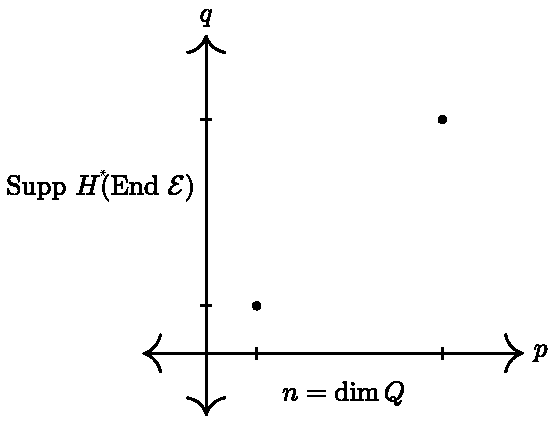
\includegraphics[width=0.5\textwidth]{spectral_sequence.pdf}
\caption{We have a range of $n$ on the $p$ axis, 
and $\Supp H^*\left( \End \cE \right)$ on the $q$ axis.}
\label{fig:spectral}
\end{figure}
Since the thing the spectral sequence is converging to,
$H^*\left( L \right)$, is defined in degree $0, \cdots , n$
as in \cref{fig:spectral},
we conclude that $H^*\left(\End \cE_L \right)$ is concentrated in a single degree,
which implies that $H^*\cE_L$ is also concentrated in a single degree.
Moreover it is one-dimensional.
So $H^*\left( L \right) = H^*Q \tp \End H^* \cE_L$. 
So if we just count ranks, we see that 
$H^* \cE_L$ has to have rank $1$

In general, one really has to use the geometry of the holomorphic curves in 
proving the Arnold conjecture,
which is fruitful in $4$-dimensions, but not so much in higher dimensions.

\end{document}
